\documentclass[tikz,border=5pt]{standalone}
\usetikzlibrary{calc,intersections}

\begin{document}
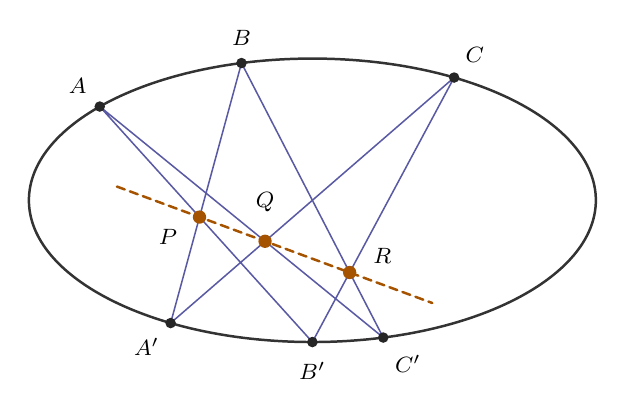
\begin{tikzpicture}[
    scale=1.8,
    line cap=round,
    line join=round,
    conic/.style={draw=black!80,line width=.9pt},
    chord/.style={draw=blue!45!black,opacity=.65,line width=.55pt},
    pascal/.style={draw=orange!65!black,line width=.9pt,
                   dash pattern=on 3pt off 2pt},
    point/.style={circle,fill=black!85,inner sep=1.35pt},
    intersection point/.style={circle,fill=orange!65!black,
                               inner sep=1.7pt},
    every label/.style={font=\footnotesize,inner sep=1pt,text=black}
]
    \coordinate (A)  at (-1.5,{sqrt(1-1.5^2/4)});
    \coordinate (B)  at (-.5,{sqrt(1-.5^2/4)});
    \coordinate (C)  at (1,{sqrt(1-1^2/4)});
    \coordinate (Ap) at (-1,{-sqrt(1-1^2/4)});
    \coordinate (Bp) at (0,-1);
    \coordinate (Cp) at (.5,{-sqrt(1-.5^2/4)});

    \path[name path=ABp] (A)--(Bp);
    \path[name path=BAp] (B)--(Ap);
    \path[name path=ACp] (A)--(Cp);
    \path[name path=CAp] (C)--(Ap);
    \path[name path=BCp] (B)--(Cp);
    \path[name path=CBp] (C)--(Bp);

    \path[name intersections={of=ABp and BAp,by=P}];
    \path[name intersections={of=ACp and CAp,by=Q}];
    \path[name intersections={of=BCp and CBp,by=R}];

    \draw[conic] (0,0) ellipse[x radius=2,y radius=1];
    \draw[chord] (A)--(Bp) (B)--(Ap)
                 (A)--(Cp) (C)--(Ap)
                 (B)--(Cp) (C)--(Bp);
    \draw[pascal] ($(P)!-.55!(R)$)--($(P)!1.55!(R)$);

    \node[point,label={[label distance=3pt]135:$A$}] at (A) {};
    \node[point,label={[label distance=3pt]90:$B$}] at (B) {};
    \node[point,label={[label distance=3pt]55:$C$}] at (C) {};
    \node[point,label={[label distance=3pt]235:$A'$}] at (Ap) {};
    \node[point,label={[label distance=4pt]270:$B'$}] at (Bp) {};
    \node[point,label={[label distance=4pt]300:$C'$}] at (Cp) {};

    \node[intersection point,label={[label distance=5pt]205:$P$}] at (P) {};
    \node[intersection point,label={[label distance=7pt]90:$Q$}] at (Q) {};
    \node[intersection point,label={[label distance=5pt]15:$R$}] at (R) {};
\end{tikzpicture}
\end{document}
